\documentclass[11pt,a4paper]{article}

\usepackage[margin=1in]{geometry}
\usepackage{mathptmx}
\usepackage{amsmath}
\usepackage{amssymb}
\usepackage{amsthm}
\usepackage{braket}
\usepackage{tikz}
\usepackage{quantikz}
\usepackage{enumitem}
\usepackage{hyperref}
\usepackage{xcolor}

\definecolor{circuitblue}{RGB}{40,80,160}

\hypersetup{
    colorlinks=true,
    linkcolor=circuitblue,
    urlcolor=circuitblue,
    citecolor=circuitblue
}

\theoremstyle{definition}
\newtheorem{definition}{Definition}[section]
\newtheorem{example}{Example}[section]

\theoremstyle{remark}
\newtheorem*{intuition}{Intuition}
\newtheorem*{keypoint}{Key Point}

\pagestyle{plain}

\setlength{\parindent}{0pt}
\setlength{\parskip}{6pt}

\begin{document}

\begin{center}
    {\LARGE \textbf{Noise in Quantum Computers (Part 1)}}\\[8pt]
    {\large QML}\\[12pt]
    \hrule
\end{center}

\vspace{12pt}
\tableofcontents
\newpage

%% ========================================================
\section{Why Noise Matters}
%% ========================================================

everything we covered so far assumed perfect quantum gates, perfect measurements, and perfect qubits that live forever. in reality, none of that is true. real quantum hardware is incredibly noisy, and understanding noise is essential for doing anything practical --- especially QML.

noise limits how deep ur circuits can be, which directly constrains the expressibility of ur quantum models. if u dont understand noise, ull build QML models that look great in simulation but produce garbage on real hardware.

\begin{keypoint}
the entire NISQ (noisy intermediate-scale quantum) era is defined by noise. every QML algorithm running on current hardware has to deal with:
\begin{itemize}
    \item gate errors ($\sim 10^{-3}$ for single qubit, $\sim 10^{-2}$ for two-qubit gates)
    \item measurement errors ($\sim 10^{-2}$)
    \item decoherence (qubits lose their quantum state over time)
    \item crosstalk (gates on one qubit affect neighboring qubits)
\end{itemize}
\end{keypoint}

%% ========================================================
\section{Sources of Noise}
%% ========================================================

\subsection{Decoherence}

\begin{definition}
\textbf{decoherence} is the process by which a qubit loses its quantum properties due to unwanted interaction with the environment. there r two timescales:
\begin{itemize}
    \item \textbf{$T_1$ (relaxation time)}: the time it takes for a qubit in $\ket{1}$ to decay to $\ket{0}$ (energy relaxation). think of it as the qubit ``falling down'' to its ground state.
    \item \textbf{$T_2$ (dephasing time)}: the time it takes for a superposition $\alpha\ket{0} + \beta\ket{1}$ to lose its phase relationship (the off-diagonal elements of the density matrix decay). always $T_2 \leq 2T_1$.
\end{itemize}
\end{definition}

\begin{intuition}
on the bloch sphere:
\begin{itemize}
    \item $T_1$ decay: the bloch vector shrinks towards the north pole ($\ket{0}$). the qubit loses energy and falls to the ground state.
    \item $T_2$ dephasing: the bloch vector shrinks towards the z-axis. the qubit loses phase information --- its no longer a coherent superposition, just a classical mixture.
\end{itemize}

typical values for superconducting qubits (IBM, Google): $T_1 \sim 50$--$300$ $\mu$s, $T_2 \sim 30$--$200$ $\mu$s. a single gate takes $\sim 20$--$100$ ns. so u get maybe $\sim 1000$ gates before decoherence kills u. for two-qubit gates ($\sim 200$--$500$ ns), the budget is even tighter.
\end{intuition}

\subsection{Gate Errors}

quantum gates r implemented by carefully timed microwave pulses (for superconducting qubits) or laser pulses (for trapped ions). imperfections in these pulses lead to gate errors:

\begin{itemize}
    \item \textbf{coherent errors}: the gate applies the wrong rotation (e.g., rotating by $\pi + \epsilon$ instead of $\pi$). these accumulate systematically.
    \item \textbf{incoherent errors}: random noise during the gate. these r modeled by quantum channels (next section).
\end{itemize}

typical gate fidelities:
\begin{center}
\begin{tabular}{l|c}
gate type & typical fidelity \\
\hline
single qubit (X, H, etc.) & $99.9\%$ ($10^{-3}$ error) \\
two-qubit (CNOT, CZ) & $99\%$--$99.5\%$ ($5 \times 10^{-3}$ to $10^{-2}$ error) \\
measurement & $97\%$--$99\%$ ($10^{-2}$ error)
\end{tabular}
\end{center}

\subsection{Measurement Errors}

measurement in quantum computing is not instantaneous or perfect. errors include:
\begin{itemize}
    \item reading $\ket{0}$ when the qubit was in $\ket{1}$ (and vice versa)
    \item the qubit decaying from $\ket{1}$ to $\ket{0}$ \textbf{during} the measurement process
    \item readout crosstalk: measuring one qubit affects the readout of neighboring qubits
\end{itemize}

\subsection{Crosstalk}

\begin{definition}
\textbf{crosstalk} occurs when an operation on one qubit unintentionally affects nearby qubits. sources include:
\begin{itemize}
    \item electromagnetic coupling between neighboring qubits
    \item shared resonators or control lines
    \item frequency collisions
\end{itemize}
\end{definition}

crosstalk is particularly nasty bcs it creates correlated errors that r harder to model and mitigate than independent errors.

%% ========================================================
\section{The Density Matrix Formalism for Noise}
%% ========================================================

\subsection{Why We Need Density Matrices}

noise turns pure states into mixed states. u cant describe a noisy quantum system with just a ket vector --- u need the density matrix formalism from lecture 1.

\begin{example}
suppose a qubit is prepared in $\ket{+} = \frac{1}{\sqrt{2}}(\ket{0} + \ket{1})$ but with some probability $p$ a bit flip error occurs. the resulting state is:
\[
\rho = (1-p)\ket{+}\bra{+} + p \cdot X\ket{+}\bra{+}X = (1-p)\ket{+}\bra{+} + p\ket{-}\bra{-}
\]
\[
= \frac{1}{2}\begin{pmatrix} 1 & 1-2p \\ 1-2p & 1 \end{pmatrix}
\]

for $p = 0$: pure $\ket{+}$ state. for $p = 1/2$: maximally mixed $I/2$. the off-diagonal elements (coherences) decay as $p$ increases.
\end{example}

%% ========================================================
\section{Quantum Channels}
%% ========================================================

\subsection{What is a Quantum Channel?}

\begin{definition}
a \textbf{quantum channel} $\mathcal{E}$ is a map from density matrices to density matrices that is:
\begin{enumerate}[label=(\roman*)]
    \item \textbf{linear}: $\mathcal{E}(\alpha\rho + \beta\sigma) = \alpha\mathcal{E}(\rho) + \beta\mathcal{E}(\sigma)$
    \item \textbf{completely positive (CP)}: maps positive operators to positive operators, even when tensored with an identity map on an ancilla
    \item \textbf{trace preserving (TP)}: $\text{tr}(\mathcal{E}(\rho)) = \text{tr}(\rho) = 1$
\end{enumerate}
together, these r called \textbf{CPTP maps}. every physical noise process is a CPTP map.
\end{definition}

\begin{intuition}
why ``completely positive'' and not just ``positive''? bcs quantum systems can be entangled with other systems. if alice's qubit is entangled with bob's, and noise acts only on alice's qubit, the combined state must still be a valid density matrix. ``completely positive'' ensures this works even for entangled states. just ``positive'' is not enough --- there exist positive but not completely positive maps (like the transpose map) that would produce non-physical states when applied to one half of an entangled pair.
\end{intuition}

\subsection{Kraus Representation}

\begin{definition}
every quantum channel $\mathcal{E}$ can be written in \textbf{Kraus form}:
\[
\boxed{\mathcal{E}(\rho) = \sum_k E_k \rho E_k^\dagger}
\]
where the \textbf{Kraus operators} $\{E_k\}$ satisfy the completeness condition:
\[
\sum_k E_k^\dagger E_k = I
\]
\end{definition}

the kraus operators r not unique --- diff sets of kraus operators can describe the same channel. but the channel itself is unique.

\begin{intuition}
each kraus operator represents one ``branch'' of the noise process. u can think of it as: with some probability, the noise applies $E_k$ to the state (and then normalizes). the completeness condition ensures probabilities sum to 1.

a unitary evolution $U$ is a special case with a single kraus operator: $\mathcal{E}(\rho) = U\rho U^\dagger$.
\end{intuition}

%% ========================================================
\section{Common Noise Models}
%% ========================================================

\subsection{Bit Flip Channel}

before we dive into the math, heres how noise looks in a circuit picture. a noisy gate can be modeled as an ideal gate followed by a noise channel:

\begin{center}
\begin{quantikz}
\lstick{$\ket{0}$} & \gate{H} & \gate[style={fill=red!20}]{\mathcal{E}} & \ctrl{1} & \gate[style={fill=red!20}]{\mathcal{E}} & \meter{} \\
\lstick{$\ket{0}$} & \qw & \qw & \targ{} & \gate[style={fill=red!20}]{\mathcal{E}} & \meter{}
\end{quantikz}
\end{center}

each red $\mathcal{E}$ block represents a noise channel applied after the ideal gate. in practice, noise hits after every gate --- so the total noise accumulates with circuit depth.

\begin{definition}
the \textbf{bit flip channel} applies $X$ with probability $p$ and does nothing with probability $1-p$:
\[
\mathcal{E}_{\text{BF}}(\rho) = (1-p)\rho + p X\rho X
\]
kraus operators: $E_0 = \sqrt{1-p}\,I$, $E_1 = \sqrt{p}\,X$.
\end{definition}

\begin{example}
apply the bit flip channel to $\ket{0}$:
\[
\mathcal{E}_{\text{BF}}(\ket{0}\bra{0}) = (1-p)\ket{0}\bra{0} + p\ket{1}\bra{1} = \begin{pmatrix} 1-p & 0 \\ 0 & p \end{pmatrix}
\]
the qubit has probability $p$ of being flipped to $\ket{1}$.
\end{example}

\begin{example}
apply the bit flip channel to $\ket{+}$:
\begin{align}
\mathcal{E}_{\text{BF}}(\ket{+}\bra{+}) &= (1-p)\frac{1}{2}\begin{pmatrix} 1 & 1 \\ 1 & 1 \end{pmatrix} + p \frac{1}{2}\begin{pmatrix} 1 & -1 \\ -1 & 1 \end{pmatrix} \\
&= \frac{1}{2}\begin{pmatrix} 1 & 1-2p \\ 1-2p & 1 \end{pmatrix}
\end{align}
the diagonal elements r unchanged but the off-diagonal elements (coherences) decay by a factor of $(1-2p)$.
\end{example}

\subsection{Phase Flip Channel}

\begin{definition}
the \textbf{phase flip channel} applies $Z$ with probability $p$:
\[
\mathcal{E}_{\text{PF}}(\rho) = (1-p)\rho + p Z\rho Z
\]
kraus operators: $E_0 = \sqrt{1-p}\,I$, $E_1 = \sqrt{p}\,Z$.
\end{definition}

\begin{example}
apply to $\ket{0}$:
\[
\mathcal{E}_{\text{PF}}(\ket{0}\bra{0}) = (1-p)\ket{0}\bra{0} + p\ket{0}\bra{0} = \ket{0}\bra{0}
\]
no effect! $\ket{0}$ is an eigenstate of $Z$, so Z errors dont affect it.
\end{example}

\begin{example}
apply to $\ket{+}$:
\begin{align}
\mathcal{E}_{\text{PF}}(\ket{+}\bra{+}) &= (1-p)\ket{+}\bra{+} + p\ket{-}\bra{-} \\
&= \frac{1}{2}\begin{pmatrix} 1 & 1-2p \\ 1-2p & 1 \end{pmatrix}
\end{align}
same result as the bit flip channel on $\ket{+}$. but different physics --- the bit flip flips the computational basis, the phase flip flips the phase.
\end{example}

\begin{keypoint}
the bit flip and phase flip channels r related by the hadamard transformation:
\[
\mathcal{E}_{\text{PF}} = H \circ \mathcal{E}_{\text{BF}} \circ H
\]
bcs $HXH = Z$. a bit flip in the X basis is a phase flip in the Z basis.
\end{keypoint}

\subsection{Bit-Phase Flip Channel}

\begin{definition}
the \textbf{bit-phase flip channel} applies $Y$ with probability $p$:
\[
\mathcal{E}_{\text{BPF}}(\rho) = (1-p)\rho + p Y\rho Y
\]
\end{definition}

since $Y = iXZ$, the bit-phase flip applies both a bit flip and a phase flip simultaneously.

\subsection{Depolarizing Channel}

\begin{definition}
the \textbf{depolarizing channel} applies each pauli error ($X$, $Y$, $Z$) with equal probability $p/3$:
\[
\boxed{\mathcal{E}_{\text{dep}}(\rho) = (1-p)\rho + \frac{p}{3}(X\rho X + Y\rho Y + Z\rho Z)}
\]
\end{definition}

equivalently:
\[
\mathcal{E}_{\text{dep}}(\rho) = \left(1 - \frac{4p}{3}\right)\rho + \frac{4p}{3} \cdot \frac{I}{2}
\]

\begin{intuition}
the depolarizing channel ``pushes'' the state towards the maximally mixed state $I/2$ (the center of the bloch sphere). with probability $1-p$, nothing happens. with probability $p$, a random pauli error occurs. at $p = 3/4$, the state is completely depolarized to $I/2$.

on the bloch sphere, the depolarizing channel uniformly shrinks the bloch vector:
\[
\vec{r} \to (1 - 4p/3)\vec{r}
\]
the bloch vector shrinks by a factor of $(1-4p/3)$ in every direction.
\end{intuition}

\begin{example}
depolarize $\ket{0}$ with $p = 0.1$:
\begin{align}
\mathcal{E}_{\text{dep}}(\ket{0}\bra{0}) &= 0.9\begin{pmatrix} 1 & 0 \\ 0 & 0 \end{pmatrix} + \frac{0.1}{3}\left[\begin{pmatrix} 0 & 0 \\ 0 & 1 \end{pmatrix} + \begin{pmatrix} 0 & 0 \\ 0 & 1 \end{pmatrix} + \begin{pmatrix} 1 & 0 \\ 0 & 0 \end{pmatrix}\right] \\
&= 0.9\begin{pmatrix} 1 & 0 \\ 0 & 0 \end{pmatrix} + \frac{0.1}{3}\begin{pmatrix} 1 & 0 \\ 0 & 2 \end{pmatrix} \\
&= \begin{pmatrix} 0.933 & 0 \\ 0 & 0.067 \end{pmatrix}
\end{align}
theres now a $6.7\%$ chance of measuring $\ket{1}$.
\end{example}

\subsection{Amplitude Damping Channel}

\begin{definition}
the \textbf{amplitude damping channel} models $T_1$ decay (energy relaxation):
\[
\mathcal{E}_{\text{AD}}(\rho) = E_0 \rho E_0^\dagger + E_1 \rho E_1^\dagger
\]
with kraus operators:
\[
E_0 = \begin{pmatrix} 1 & 0 \\ 0 & \sqrt{1-\gamma} \end{pmatrix}, \quad E_1 = \begin{pmatrix} 0 & \sqrt{\gamma} \\ 0 & 0 \end{pmatrix}
\]
where $\gamma = 1 - e^{-t/T_1}$ is the damping probability.
\end{definition}

\begin{intuition}
amplitude damping models the physical process of a qubit losing energy to its environment. $\ket{1}$ decays to $\ket{0}$ with probability $\gamma$ (per time step). $\ket{0}$ is unaffected bcs its already the ground state.

$E_0$ describes the ``no decay'' outcome: the $\ket{0}$ component is unchanged, the $\ket{1}$ component gets reduced by $\sqrt{1-\gamma}$.

$E_1$ describes the ``decay'' outcome: $\ket{1}$ transitions to $\ket{0}$.
\end{intuition}

\begin{example}
apply amplitude damping to $\ket{1}$:
\begin{align}
\mathcal{E}_{\text{AD}}(\ket{1}\bra{1}) &= E_0\ket{1}\bra{1}E_0^\dagger + E_1\ket{1}\bra{1}E_1^\dagger \\
&= (1-\gamma)\ket{1}\bra{1} + \gamma\ket{0}\bra{0} \\
&= \begin{pmatrix} \gamma & 0 \\ 0 & 1-\gamma \end{pmatrix}
\end{align}
the qubit has probability $\gamma$ of decaying to $\ket{0}$.
\end{example}

\begin{example}
apply amplitude damping to $\ket{+}$:
\begin{align}
\rho_{\text{in}} &= \ket{+}\bra{+} = \frac{1}{2}\begin{pmatrix} 1 & 1 \\ 1 & 1 \end{pmatrix} \\[6pt]
E_0\rho E_0^\dagger &= \frac{1}{2}\begin{pmatrix} 1 & \sqrt{1-\gamma} \\ \sqrt{1-\gamma} & 1-\gamma \end{pmatrix} \\[6pt]
E_1\rho E_1^\dagger &= \frac{1}{2}\begin{pmatrix} \gamma & 0 \\ 0 & 0 \end{pmatrix} \\[6pt]
\mathcal{E}_{\text{AD}}(\rho) &= \frac{1}{2}\begin{pmatrix} 1+\gamma & \sqrt{1-\gamma} \\ \sqrt{1-\gamma} & 1-\gamma \end{pmatrix}
\end{align}
both the populations and coherences r affected. as $\gamma \to 1$, the state approaches $\ket{0}\bra{0}$.
\end{example}

\subsection{Phase Damping (Dephasing) Channel}

\begin{definition}
the \textbf{phase damping channel} models $T_2$ dephasing:
\[
\mathcal{E}_{\text{PD}}(\rho) = E_0 \rho E_0^\dagger + E_1 \rho E_1^\dagger
\]
with:
\[
E_0 = \begin{pmatrix} 1 & 0 \\ 0 & \sqrt{1-\lambda} \end{pmatrix}, \quad E_1 = \begin{pmatrix} 0 & 0 \\ 0 & \sqrt{\lambda} \end{pmatrix}
\]
where $\lambda = 1 - e^{-t/T_2}$.
\end{definition}

\begin{example}
apply to a general state $\rho = \begin{pmatrix} \rho_{00} & \rho_{01} \\ \rho_{10} & \rho_{11} \end{pmatrix}$:
\[
\mathcal{E}_{\text{PD}}(\rho) = \begin{pmatrix} \rho_{00} & \sqrt{1-\lambda}\,\rho_{01} \\ \sqrt{1-\lambda}\,\rho_{10} & \rho_{11} \end{pmatrix}
\]
the diagonal elements (populations) r unchanged. only the off-diagonal elements (coherences) decay by $\sqrt{1-\lambda}$.
\end{example}

\begin{keypoint}
comparison of noise channels and their effects:
\begin{center}
\begin{tabular}{l|c|c}
channel & populations & coherences \\
\hline
bit flip & affected & decay by $(1-2p)$ \\
phase flip & unchanged & decay by $(1-2p)$ \\
depolarizing & pushed towards $1/2$ & decay by $(1-4p/3)$ \\
amplitude damping & $\ket{1} \to \ket{0}$ & decay by $\sqrt{1-\gamma}$ \\
phase damping & unchanged & decay by $\sqrt{1-\lambda}$
\end{tabular}
\end{center}
\end{keypoint}

%% ========================================================
\section{Fidelity and Trace Distance}
%% ========================================================

\subsection{Fidelity}

how do we measure how close a noisy state is to the ideal state? two main measures:

\begin{definition}
the \textbf{fidelity} between two quantum states $\rho$ and $\sigma$ is:
\[
\boxed{F(\rho, \sigma) = \left(\text{tr}\sqrt{\sqrt{\rho}\,\sigma\sqrt{\rho}}\right)^2}
\]
for a pure state $\ket{\psi}$ and a mixed state $\rho$, this simplifies to:
\[
F(\ket{\psi}, \rho) = \bra{\psi}\rho\ket{\psi}
\]
\end{definition}

properties:
\begin{itemize}
    \item $0 \leq F \leq 1$
    \item $F = 1$ iff $\rho = \sigma$
    \item $F = 0$ iff $\rho$ and $\sigma$ have orthogonal supports
    \item $F$ is symmetric: $F(\rho, \sigma) = F(\sigma, \rho)$
\end{itemize}

\begin{example}
fidelity between $\ket{0}$ and a noisy state $\rho = \begin{pmatrix} 1-\epsilon & 0 \\ 0 & \epsilon \end{pmatrix}$:
\[
F = \bra{0}\rho\ket{0} = 1 - \epsilon
\]
\end{example}

\subsection{Average Gate Fidelity}

\begin{definition}
the \textbf{average gate fidelity} of a noisy gate $\mathcal{E}$ compared to the ideal gate $U$ is:
\[
\bar{F}(\mathcal{E}, U) = \int d\psi \, \bra{\psi} U^\dagger \mathcal{E}(\ket{\psi}\bra{\psi}) U \ket{\psi}
\]
where the integral is over the uniform (Haar) measure on pure states.
\end{definition}

this is the number u see reported in hardware benchmarks. a gate fidelity of $99.9\%$ means the average error per gate is $0.1\%$.

\subsection{Trace Distance}

\begin{definition}
the \textbf{trace distance} between $\rho$ and $\sigma$ is:
\[
\boxed{D(\rho, \sigma) = \frac{1}{2}\|\rho - \sigma\|_1 = \frac{1}{2}\text{tr}\sqrt{(\rho - \sigma)^\dagger(\rho - \sigma)}}
\]
for single-qubit states, this simplifies to half the sum of absolute eigenvalues of $\rho - \sigma$.
\end{definition}

\begin{keypoint}
the trace distance has a beautiful operational interpretation: its the maximum probability of distinguishing $\rho$ from $\sigma$ using any measurement, minus $1/2$:
\[
D(\rho, \sigma) = \max_{\text{measurements}} \left|P(\text{outcome}|\rho) - P(\text{outcome}|\sigma)\right|
\]
if $D = 0$, the states r identical and no measurement can tell them apart. if $D = 1$, the states r perfectly distinguishable.
\end{keypoint}

\begin{example}
trace distance between $\ket{0}$ and $\ket{1}$:
\[
\rho - \sigma = \begin{pmatrix} 1 & 0 \\ 0 & -1 \end{pmatrix}
\]
eigenvalues: $+1, -1$. trace distance: $\frac{1}{2}(1 + 1) = 1$. perfectly distinguishable.
\end{example}

\begin{example}
trace distance between $\ket{0}$ and $\ket{+}$:
\[
\rho - \sigma = \begin{pmatrix} 1 & 0 \\ 0 & 0 \end{pmatrix} - \frac{1}{2}\begin{pmatrix} 1 & 1 \\ 1 & 1 \end{pmatrix} = \frac{1}{2}\begin{pmatrix} 1 & -1 \\ -1 & -1 \end{pmatrix}
\]
eigenvalues of $(\rho - \sigma)$: $\pm \frac{1}{\sqrt{2}}$. trace distance: $\frac{1}{2}(\frac{1}{\sqrt{2}} + \frac{1}{\sqrt{2}}) = \frac{1}{\sqrt{2}} \approx 0.707$.
\end{example}

\subsection{Relation Between Fidelity and Trace Distance}

for any two states:
\[
1 - \sqrt{F(\rho, \sigma)} \leq D(\rho, \sigma) \leq \sqrt{1 - F(\rho, \sigma)}
\]

so high fidelity ($F \approx 1$) implies small trace distance ($D \approx 0$) and vice versa. but they r not simple functions of each other.

%% ========================================================
\section{How Noise Affects Circuit Output}
%% ========================================================

\subsection{Error Accumulation}

for a circuit with $d$ gates, each with error probability $\epsilon$, the total error grows roughly as:
\[
\text{total error} \approx d \cdot \epsilon
\]

this is a rough bound. the actual error depends on the circuit structure, error correlations, and whether errors cancel or compound.

\begin{center}
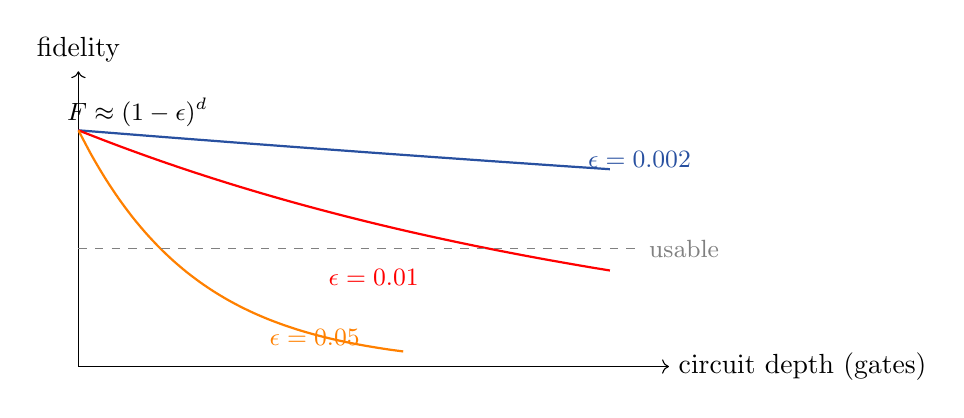
\begin{tikzpicture}[scale=0.75]
    \draw[->] (0,0) -- (10,0) node[right] {circuit depth (gates)};
    \draw[->] (0,0) -- (0,5) node[above] {fidelity};

    % fidelity decay curves
    \draw[thick, circuitblue, domain=0:9, smooth] plot (\x, {4*exp(-0.02*\x)});
    \node[circuitblue] at (9.5, 3.5) {\small $\epsilon=0.002$};

    \draw[thick, red, domain=0:9, smooth] plot (\x, {4*exp(-0.1*\x)});
    \node[red] at (5, 1.5) {\small $\epsilon=0.01$};

    \draw[thick, orange, domain=0:5.5, smooth] plot (\x, {4*exp(-0.5*\x)});
    \node[orange] at (4, 0.5) {\small $\epsilon=0.05$};

    % useful threshold
    \draw[dashed, gray] (0, 2) -- (9.5, 2);
    \node[gray, right] at (9.5, 2) {\small usable};

    \node at (1, 4.3) {\small $F \approx (1-\epsilon)^d$};
\end{tikzpicture}
\end{center}

\begin{keypoint}
practical circuit depth limits on current hardware:
\begin{itemize}
    \item CNOT fidelity $\sim 99\%$ ($\epsilon \sim 0.01$)
    \item for the output to be meaningful, need total error $\lesssim 0.5$
    \item max useful circuit depth: $\sim 50$--$100$ two-qubit gates
    \item beyond this, output is basically random noise
\end{itemize}
this severely constrains QML: ur quantum model cant be too deep. this is why hardware-efficient ansatze and shallow circuits r so important.
\end{keypoint}

\subsection{Noise in Expectation Values}

in variational algorithms (including QML), we typically measure expectation values $\langle O \rangle = \text{tr}(O\rho)$. noise shifts these:

for the depolarizing channel with parameter $p$ applied to each gate, after $d$ gates:
\[
\langle O \rangle_{\text{noisy}} \approx (1 - p)^d \langle O \rangle_{\text{ideal}} + (1 - (1-p)^d) \cdot \text{tr}(O \cdot I/2^n)
\]

the signal decays exponentially with circuit depth: $(1-p)^d \approx e^{-pd}$.

\begin{intuition}
noise pushes expectation values towards their ``maximally mixed'' value. for a pauli observable $O$ with eigenvalues $\pm 1$, the maximally mixed expectation value is 0. so noise \textbf{exponentially suppresses} the signal in ur quantum circuit. this is one of the fundamental challenges of NISQ computing.
\end{intuition}

\subsection{Noise in Probability Distributions}

if the ideal output distribution is $p_{\text{ideal}}(x)$ and the noisy distribution is $p_{\text{noisy}}(x)$:
\[
p_{\text{noisy}}(x) = (1-\epsilon) p_{\text{ideal}}(x) + \epsilon \cdot p_{\text{uniform}}(x)
\]

where $\epsilon$ is the total error. the noisy distribution is a mixture of the ideal distribution and uniform random noise.

%% ========================================================
\section{Pauli Transfer Matrix Representation}
%% ========================================================

\begin{definition}
any single-qubit channel can be represented as a $4 \times 4$ \textbf{Pauli transfer matrix} (PTM) acting on the pauli coefficient vector $(c_I, c_X, c_Y, c_Z)$ where $\rho = \frac{1}{2}(c_I I + c_X X + c_Y Y + c_Z Z)$.
\end{definition}

\begin{example}
the depolarizing channel PTM:
\[
\Lambda_{\text{dep}} = \begin{pmatrix} 1 & 0 & 0 & 0 \\ 0 & 1-4p/3 & 0 & 0 \\ 0 & 0 & 1-4p/3 & 0 \\ 0 & 0 & 0 & 1-4p/3 \end{pmatrix}
\]
the identity coefficient is preserved (trace preservation), and all pauli coefficients r uniformly damped.
\end{example}

\begin{example}
the amplitude damping channel PTM (with parameter $\gamma$):
\[
\Lambda_{\text{AD}} = \begin{pmatrix} 1 & 0 & 0 & 0 \\ 0 & \sqrt{1-\gamma} & 0 & 0 \\ 0 & 0 & \sqrt{1-\gamma} & 0 \\ \gamma & 0 & 0 & 1-\gamma \end{pmatrix}
\]
note the asymmetry: x and y bloch vector components decay as $\sqrt{1-\gamma}$, the z component decays as $1-\gamma$ and shifts by $\gamma$ (towards $\ket{0}$).
\end{example}

%% ========================================================
\section{Noise Channels on the Bloch Sphere}
%% ========================================================

a nice way to visualize noise is by its effect on the bloch sphere. each noise channel maps the bloch sphere to a (possibly deformed) ellipsoid:

\begin{center}
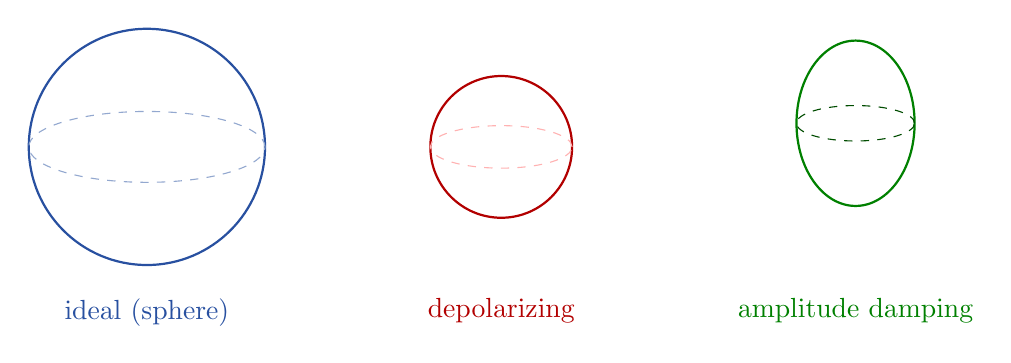
\begin{tikzpicture}[scale=1.5]
    % original sphere
    \draw[thick, circuitblue] (0,0) circle (1);
    \draw[dashed, circuitblue!50] (0,0) ellipse (1 and 0.3);
    \node[circuitblue, below] at (0,-1.2) {ideal (sphere)};

    % depolarizing
    \begin{scope}[xshift=3cm]
    \draw[thick, red!70!black] (0,0) circle (0.6);
    \draw[dashed, red!30] (0,0) ellipse (0.6 and 0.18);
    \node[red!70!black, below] at (0,-1.2) {depolarizing};
    \end{scope}

    % amplitude damping
    \begin{scope}[xshift=6cm]
    \draw[thick, green!50!black] (0,0.2) ellipse (0.5 and 0.7);
    \draw[dashed, green!30!black] (0,0.2) ellipse (0.5 and 0.15);
    \node[green!50!black, below] at (0,-1.2) {amplitude damping};
    \end{scope}
\end{tikzpicture}
\end{center}

\begin{itemize}
    \item \textbf{depolarizing}: uniform shrinking (sphere $\to$ smaller sphere)
    \item \textbf{amplitude damping}: asymmetric shrinking + shift towards $\ket{0}$ (sphere $\to$ shifted ellipsoid)
    \item \textbf{phase damping}: shrinking in the x-y plane only (sphere $\to$ oblate ellipsoid)
\end{itemize}

%% ========================================================
\section{Choi-Jamiolkowski Isomorphism}
%% ========================================================

theres a beautiful mathematical fact that connects quantum channels to quantum states:

\begin{definition}
the \textbf{Choi matrix} of a channel $\mathcal{E}$ acting on $d$-dimensional systems is:
\[
J(\mathcal{E}) = \sum_{i,j=0}^{d-1} \ket{i}\bra{j} \otimes \mathcal{E}(\ket{i}\bra{j})
\]
\end{definition}

this is a $d^2 \times d^2$ matrix. the channel $\mathcal{E}$ is completely positive iff $J(\mathcal{E})$ is positive semidefinite. trace preservation corresponds to a partial trace condition.

\begin{intuition}
the choi matrix lets u represent a quantum channel as a quantum state (of a doubled system). this is incredibly useful for characterizing noise channels experimentally --- instead of probing the channel with many diff inputs, u can prepare a maximally entangled state, send one half through the channel, and do quantum state tomography on the output. the resulting state IS the choi matrix.
\end{intuition}

%% ========================================================
\section{Summary}
%% ========================================================

\begin{keypoint}
the key takeaways:
\begin{enumerate}
    \item real quantum computers r noisy --- decoherence, gate errors, measurement errors, crosstalk
    \item $T_1$ (relaxation) and $T_2$ (dephasing) set the fundamental timescales
    \item noise is described by quantum channels (CPTP maps) with kraus operator representation
    \item common noise models: bit flip, phase flip, depolarizing, amplitude damping, phase damping
    \item fidelity and trace distance measure how close noisy states r to ideal states
    \item noise causes exponential signal decay with circuit depth
    \item for QML: noise limits circuit depth, which limits model expressibility. designing noise-aware QML models is essential
\end{enumerate}
\end{keypoint}

next lecture: how to fight back against noise --- error mitigation techniques that make NISQ devices actually useful.

\end{document}
